\chapter{Formal analysis}
\section{Alloy formal analysis}

In this section is described a formal analysis written using Alloy. The purpose of the analysis is to highlight the key model relationships and the main constraints of the system. \\

The model has been built following the class diagram, the included code contains all the models and the relationships, and it shows that the resulting system is feasible and useful and it justifies our modelling decisions.\\

In the following sections you will find the code used to run the analysis and some of the world that the Alloy tools generated from our definitions.

\clearpage
\newpage

\section{Alloy code}

\definecolor{dkgreen}{rgb}{0,0.6,0}
\definecolor{gray}{rgb}{0.5,0.5,0.5}
\definecolor{mauve}{rgb}{0.58,0,0.82}

\lstset{frame=tb,
  language=Alloy,
  aboveskip=3mm,
  belowskip=3mm,
  showstringspaces=false,
  columns=flexible,
  basicstyle={\small\ttfamily},
  numbers=none,
  numberstyle=\tiny\color{gray},
  keywordstyle=\color{blue},
  commentstyle=\color{dkgreen},
  stringstyle=\color{mauve},
  breaklines=true,
  breakatwhitespace=true,
  tabsize=3
}


\begin{lstlisting}

//FILE: alloy_eMSP.als

//abstract sig String {} -- commented as the used version of Alloy includes it
abstract sig Bool {}
one sig TRUE extends Bool {}
one sig FALSE extends Bool {}


sig ConnectorType {}
sig Device {} {
	(one u: User | this in u.devices) and -- device needs a user
	(no disj u, u': User | this in u.devices & u'.devices) -- no device can be owned by multiple users
}

sig LicensePlate {} {
	(one v: Vehicle | v.licensePlate = this) -- licence is used only as string here so cannot exists without a vehicle
}
sig Vehicle {
	licensePlate: one LicensePlate,
	connector: one ConnectorType
} {
	(one u: User | this in u.vehicles) and -- vehicle needs a user
	(no disj u, u': User | this in u.vehicles & u'.vehicles) -- no vehicle can be owned by multiple users
}

sig User {
	devices: set Device,
	vehicles: set Vehicle,
	bookings: set Booking
} {
	#devices > 0 and #vehicles > 0
}


sig CPMS {
	chargingPoints: set ChargingPoint,
	tariffs: set Tariff,
} {
 	(#chargingPoints) > 0 and
	(#tariffs > 0)
}

sig ChargingSocket {
	isFast: one Bool,
	connectorType: one ConnectorType
} {
	(one slot: ChargingSlot | this in slot.sockets) and -- sockets needs to have one slot connected
	(no disj s, s': ChargingSlot | this in s.sockets & s'.sockets) -- no multiple slots for the same socket
}

sig ChargingSlot {
	sockets: set ChargingSocket
} {
	(one cp: ChargingPoint | this in cp.chargingSlots) and -- charging slot needs to be in a charging point
	(no disj cp, cp': ChargingPoint | this in cp.chargingSlots & cp'.chargingSlots) and -- a charging slot cannot be in multiple charging points
	(#sockets > 0)
}

sig ChargingPoint {
	chargingSlots: set ChargingSlot
} {
	 (one cpms: CPMS | this in cpms.chargingPoints) and -- charging point needs a CPMS
	 (no disj cpms, cpms': CPMS | this in cpms.chargingPoints & cpms'.chargingPoints) and -- charging point cannot have multiple CPMS
	 (#chargingSlots > 0)
}

sig Tariff {
	startAt: one Int,
	fastCharge: one Bool,
} {
 	(startAt > 0) and  -- dates as timestamps so they need to be > 0
	(one cpms: CPMS | this in cpms.tariffs) and -- tariff needs a CPMS
	(no disj c, c': CPMS | this in c.tariffs & c'.tariffs) -- no tariff can be used for multiple CPMS
}

sig BookingStatus {
	
}

sig Booking {
	status: one BookingStatus,
	vehicle: one Vehicle,
	slot: one ChargingSlot,
	payments: set Payment
} {
	(one user: User | this in user.bookings and vehicle in user.vehicles) and -- booking needs a user and vehicle must be owned by the same user
	(no disj u, u': User | this in u.bookings & u'.bookings) and
	(no disj p, p': payments | p.status.isFinal = TRUE and p'.status.isFinal = TRUE) -- only one successful payment must happen for a single booking
}

sig PaymentStatus {
	isFinal: one Bool
}
sig PaymentType {}

sig PaymentProvider {
	payments: set Payment
}

sig Payment {
	timestamp: one Int,
	status: PaymentStatus,
	type: PaymentType
} {
	(timestamp > 0) and
	(one provider: PaymentProvider | this in provider.payments) and -- payment needs a provider
	(no disj p, p': PaymentProvider | this in p.payments & p'.payments) and -- only one provider per payment
	(one booking: Booking | this in booking.payments) and -- payment needs a booking
	(no disj b, b': Booking | this in b.payments & b'.payments) -- only one booking for payment
}

/** ---- FACTS ---- */
fact noDifferentVehiclesWithSameLicensePlate {
	no disj v, v': Vehicle |
		v.licensePlate = v'.licensePlate
}

fact noPaymentsAfterASuccessfulOne {
	no disj p, p': Payment | (
		p.timestamp < p'.timestamp 
		and p.status.isFinal = TRUE
	)
}

fact noMultiplePricingActiveAtTheSameTimeForTheSameCPMS {
	all cpms: CPMS | (
		no disj t, t': cpms.tariffs | (
			t.startAt = t'.startAt and
			t.fastCharge = t'.fastCharge
		)
	)
}

/** ---- ASSERTIONS ---- */
assert deviceHasOneUser {
	no d: Device, u, u': User |	
		u != u' and
		d in u.devices and d in u'.devices
	and
	all d: Device |
		one u: User | d in u.devices
}

check deviceHasOneUser

assert bookingHasOnlyOnePaymentWithFinalStatus {
	all b: Booking |
		no p, p': Payment | (p != p' and p in b.payments and p' in b.payments and 
			p.status.isFinal = TRUE and p'.status.isFinal = TRUE
		)
}

check bookingHasOnlyOnePaymentWithFinalStatus

assert noMultiplePricingActiveAtTheSameTimeForTheSameCPMS {
	no disj t, t': Tariff | (
		t.~tariffs = t'.~tariffs and t.startAt = t'.startAt and t.fastCharge = t'.fastCharge
	)
}

check noMultiplePricingActiveAtTheSameTimeForTheSameCPMS

/** ---- PREDICATES ---- */

pred noCPMSInsertedWorld {
	#User > 0 and
	#CPMS = 0
}
run noCPMSInsertedWorld for 5

pred world1 {
	#User = 1
	#Payment  > 0
}
run world1 for 5

pred world2 {
	#User > 1 and
	#CPMS > 1 and
	#Booking > 1 and
	#Payment  > 1 and
	(some b: Booking | #b.payments > 1 and one p: b.payments | p.status.isFinal = TRUE) and
	(some cpms: CPMS | #cpms.tariffs > 1)
}
run world2 for 5
\end{lstlisting}


\begin{figure}[h]
\centering
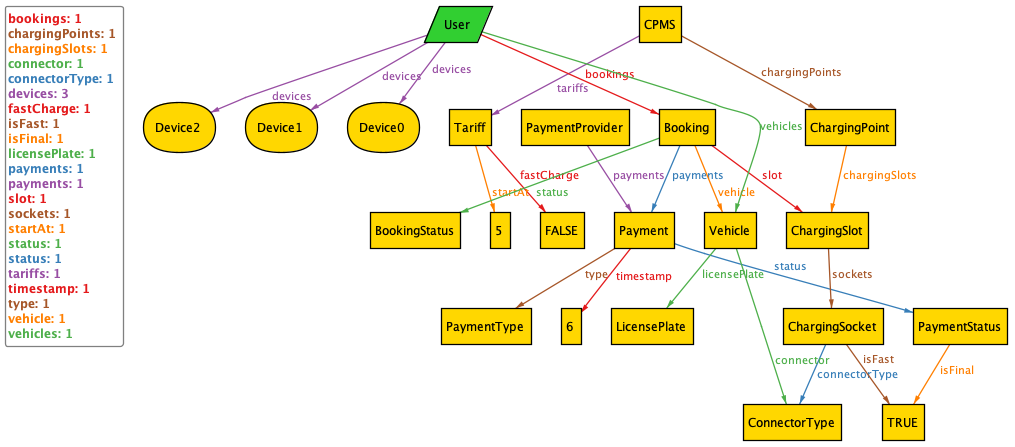
\includegraphics[width=\textwidth]{alloy/world1}
\caption{World generated by Alloy (world1) - Basic world with one user}
\end{figure}

\begin{figure}[h]
\centering
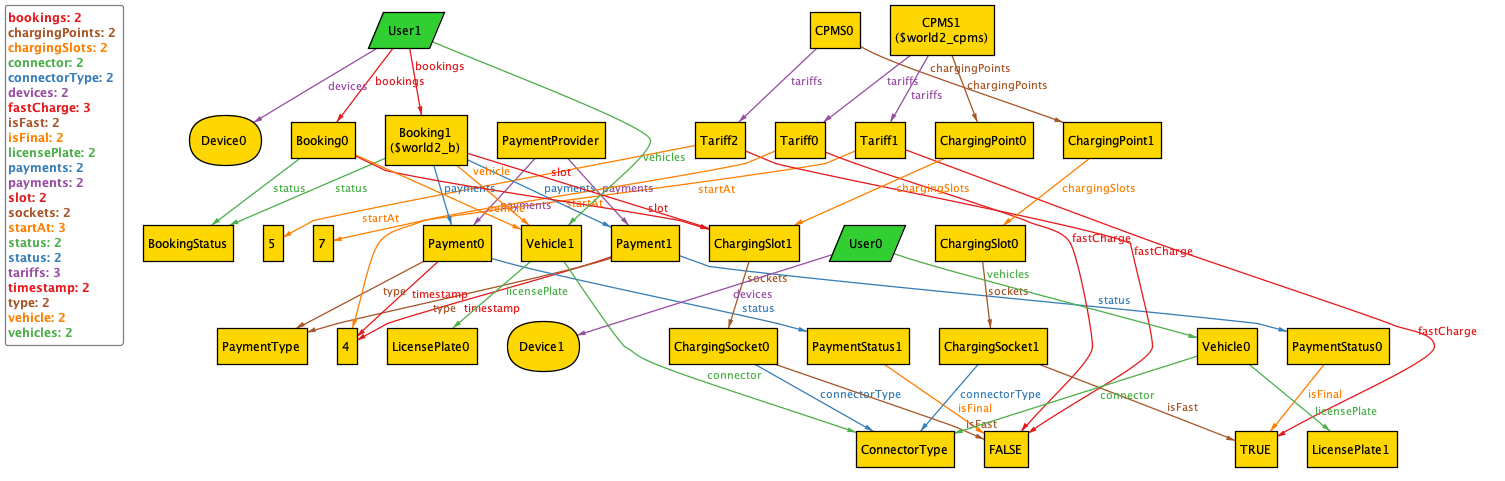
\includegraphics[width=\textwidth]{alloy/world2}
\caption{World generated by Alloy (world2) - Advanced world with multiple CPMS}
\end{figure}















